\documentclass[../p051main.tex]{subfiles}
\graphicspath{{\subfix{../figures/}}}

\begin{document}

\chapter{Magnetostatics}
\section{Current}
In our study of electrostatics, we assumed that all charges were basically stationary.
In this static equilibrium, we have $E = 0$ and a lack of net charge inside of conductors.
But in dynamic situations, charge may move more persistently!

Consider a wire with some charge flowing through it.
The rate at which charge passes through a given cross section of the wire is called the current
\[ i = \frac{dq}{dt} \]
at that point, measured in amperes (A).
To account for scenarios in which the flow of charge is not uniform over the full cross section, we can define a current density $\mbf{j}$ via
\[ i = \iint \mbf{j} \cdot d\mbf{A}, \]
where $\mbf{j}$ points in the direction of positive charge flow.
Of course we now know that it's actually negative charges (electrons) that're moving, but we stick to this convention because it isn't really hurting anyone.

Speaking of which, when we say that negative charge moves throughout a wire, we don't actually mean that electrons are rocketing through the wire at relativistic speeds, all in the same direction.
In reality their motion is much more gas-like, bouncing around with high velocities that mostly cancel each other out.
The component that does not cancel is called the drift velocity $\mbf{v}_d$, and it tends to be quite slow, on the order of one millimeter per second.
This is what creates a net movement of charge.

Now, in order to maintain this steady current throughout the wire, the electrons must be generally drifting at a constant speed.
There are two things making this happen: there is a nonzero electric field in the wire pushing the electrons along, and there is some ``drag'' force keeping the electrons from accelerating.
The forces due to these two cancel at the terminal velocity $\mbf{v}_d$.

The drift velocity is related to the current density via the equation $\mbf{j} = \rho \mbf{v}_d$, where $\rho$ is the charge density in the wire.
If we make the simplest possible assumption that the drift velocity is proportional to the electric field, we get
\[ \mbf{j} = \sigma \mbf{E}. \]
This is called Ohm's law.
Specifically, this is its intensive form since it does not depend on any of the wire's geometric properties like length or radius.
The quantity $\sigma$ is called conductivity, and it quantifies how well a material can conduct current per unit electric field.
(Its inverse $\sigma^{-1}$ is called resistivity.)

This relationship is useful, but we can use it to derive something that might be more familiar.
Suppose, now, that our wire has length $L$ and cross-sectional area $A$.
Since there is an electric field $\mbf{E}$ in the wire, there is a potential difference $\Delta V$ between the two ends; assuming constant $\mbf{E}$ and $\sigma$,
\[ \Delta V = \left| \int_{x = 0}^{x = L} \mbf{E} \cdot d\mbf{s} \right| = \left| \int_{0}^{L} \frac{j}{\sigma} dx \right| = \frac{jL}{\sigma}. \]
Since $j = i / A$, we have
\[ \Delta V = i \left( \frac{L}{\sigma A} \right) = iR, \]
where we've defined the resistance $R$, measured in ohms ($\Omega$).
This is the extensive form of Ohm's law---note that $R$ depends on the geometric properties of the wire.
Devices that are created for the purpose of providing resistance are called resistors.

\section{Circuits}
\parbox{0.65\textwidth}{
    Using wires, we can connect resistors, capacitors, and batteries (voltage sources) together to make current flow in ways that are practically useful to us.
    Schematics like the one at left are particularly useful abstractions when we want to work with circuits mathematically, like we will here.

    \vspace{6pt}
    Each circuit element is labeled with a corresponding quantity.
    The resistor has a resistance $R$, the capacitor a capacitance $C$, and the battery a voltage $V_0$.
    The battery dictates the direction of current flow---it pushes charge from low potential toward high potential, causing charge to move clockwise about the circuit.
    Right next to the battery is a switch; when closed current is allowed to flow, but when opened there is nowhere for the charge to go and the current ceases.

    \vspace{6pt}
    There are two key rules that we can exploit to ``solve'' a circuit.
}\parbox{0.35\textwidth}{
    \quad\;
    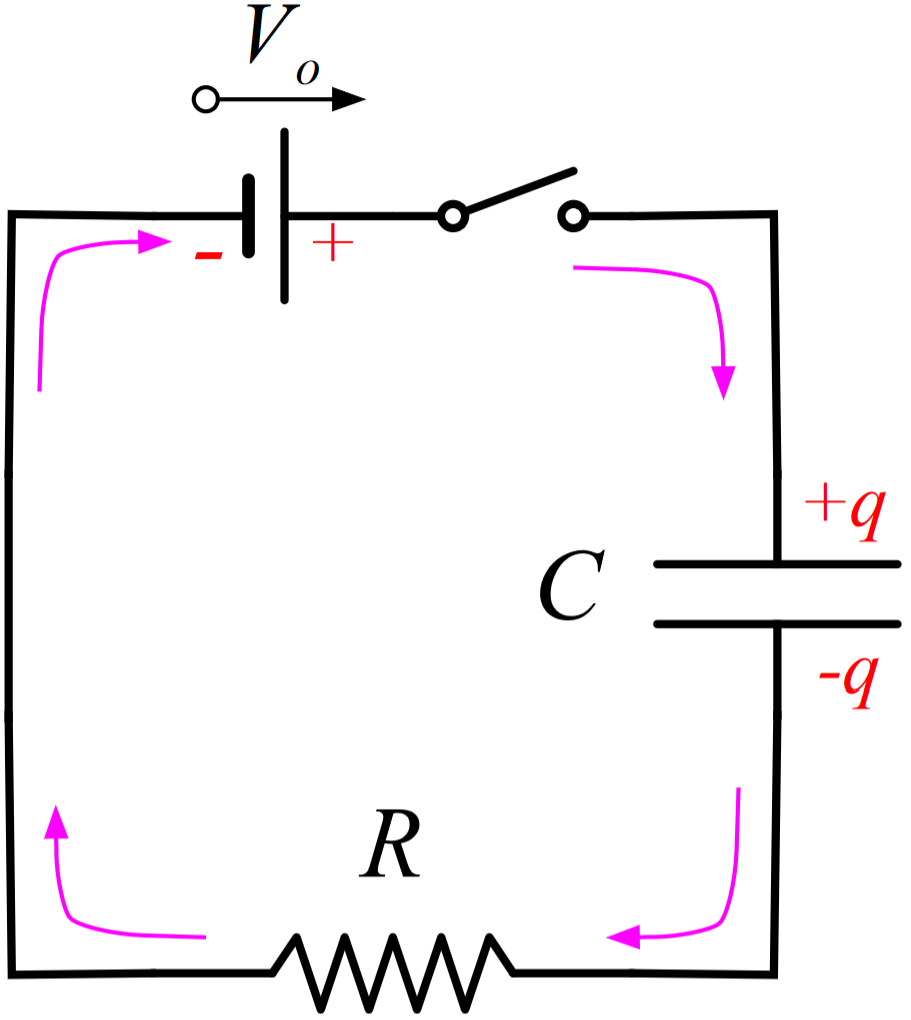
\includegraphics[width=0.3\textwidth]{rcCircuit.png}
}
\begin{itemize}
    \item By conservation of energy, the net change in potential over any loop in the circuit must be zero.
    For these purposes we can ignore any drop in potential due to travel in a wire, since it will be negligibly small compared to the potential differences across the primary circuit elements.

    \item By conservation of charge, the total current flowing into any node (any place where two wires meet) must equal the current leaving it.
\end{itemize}
Using these two rules, we are usually able to construct a system of equations that, when solved, gives the current and potential difference across each circuit element present.
We can also use them to find some convenient rules about combining like circuit elements together.
For example, we could show that pairs of resistors in parallel or in series have respective equivalent resistances
\[ R_\textrm{par} = \left( \frac{1}{R_1} + \frac{1}{R_2} \right)^{-1}, \qquad R_\textrm{ser} = R_1 + R_2. \]
We can be a bit more sophisticated, too, and examine the behavior of circuits over time.
This is especially useful in seeing, for example, how the charge on a capacitor changes while charging or discharging.

\begin{example}[Charging an RC circuit]
    Consider the above circuit.
    By conservation of energy, when the switch is closed we have
    \[ V_0 = iR + \frac{q}{C}. \]
    We can express this as a differential equation in $q(t)$, the charge on the capacitor:
    \[ \frac{dq}{dt} + \frac{1}{RC}q = \frac{V_0}{R}. \]
    With the initial condition $q(0) = 0$, the solution is
    \[ q(t) = CV_0 \left( 1 - e^{-t / RC} \right). \]
    As more charge gets deposited onto the positive plate of the capacitor, it becomes more difficult to push charge off of the other plate, around the circuit, and back onto the positive plate.
\end{example}

Finally, in order to keep the current flowing, the battery must do work on the charge to move them to higher potentials.
This work is, of course, given by $W = qV_0$, corresponding to a power
\[ P_\textrm{battery} = \frac{dW}{dt} = iV_0. \]
The resistor does an equal amount of work, so by Ohm's law we have
\[ P_\textrm{resistor} = \frac{V_0^2}{R} = i^2R \]
dissipated as heat.

% \section{Magnetic Fields}

\end{document}